\documentclass[letterpaper]{article} % DO NOT CHANGE THIS
\usepackage[submission]{aaai2027}  % DO NOT CHANGE THIS
\usepackage[hyphens]{url}  % DO NOT CHANGE THIS
\usepackage{graphicx} % DO NOT CHANGE THIS
\urlstyle{rm} % DO NOT CHANGE THIS
\def\UrlFont{\rm}  % DO NOT CHANGE THIS
\usepackage{natbib}  % DO NOT CHANGE THIS AND DO NOT ADD ANY OPTIONS TO IT
\usepackage{caption} % DO NOT CHANGE THIS AND DO NOT ADD ANY OPTIONS TO IT
\frenchspacing  % DO NOT CHANGE THIS
\usepackage{algorithm}
\usepackage{algorithmic}
\usepackage{newfloat}
\usepackage{listings}
\usepackage[htt]{hyphenat}
\usepackage{multirow}
\usepackage{makecell}
\usepackage{xcolor}
\usepackage{colortbl}
\usepackage{booktabs}

\DeclareCaptionStyle{ruled}{labelfont=normalfont,labelsep=colon,strut=off}
\lstset{%
	basicstyle={\footnotesize\ttfamily},
	numbers=left,numberstyle=\footnotesize,xleftmargin=2em,
	aboveskip=0pt,belowskip=0pt,
	showstringspaces=false,tabsize=2,breaklines=true}
\floatstyle{ruled}
\newfloat{listing}{tb}{lst}{}
\floatname{listing}{Listing}

\pdfinfo{
/TemplateVersion (2027.1)
}

\setcounter{secnumdepth}{2}

% Appendix-style section labels (A, B, C, ...)
\renewcommand{\thesection}{\Alph{section}}

\title{Supplementary Material\\
RareAgentBench: An Agent-Native Benchmark for Rare-Disease Diagnosis}
\author{}
\affiliations{}

\begin{document}
\maketitle

\noindent
This document is the supplementary material for \emph{RareAgentBench}. It is
self-contained: each appendix restates the setup it needs, so it can be read
without the main paper. It documents (A)~the data layers and their construction,
(B)~the backbone configurations, (C)~the agent fairness matrix and adapter
patches, (D)~per-baseline reproduction against published claims,
(E)~the temporal-holdout protocol, (F)~the pre-registered hypotheses and their
family-wise test results, (G)~the full cost accounting, (H)~a
MIMIC-IV note probe with a 24-cell agent matrix, and (I)~bootstrap and
reproducibility notes. Unless stated otherwise, the primary metric is
cross-ontology Recall@1 (R@1) with an \emph{attempted} denominator: every empty
output, parser error, and timeout is counted as a miss, never dropped. Disease
predictions are matched by exact identifier, then accepted OMIM--ORPHA mappings,
then Orphanet name/synonym match with a RapidFuzz threshold of 90.

% ======================================================================
\section{Data Layers and Construction}
\label{app:data}

RareAgentBench draws on a source pool of 84,450 candidate instances from five
sources, organized into four layers that vary evidence structure, clinical
realism, scale, and contamination risk. Table~\ref{tab:datalayers} summarizes the
layers as evaluated in this release; the per-layer counts are the released sizes
and do not sum to the candidate pool.

\begin{table}[h]
\centering
\scriptsize
\setlength{\tabcolsep}{3.5pt}
\caption{Data layers. ``Input'' is the evidence an agent receives; ``Gold'' is
the reference label source. Counts are released-pool sizes; per-experiment
evaluated $N$ is reported per cell in the main paper.}
\label{tab:datalayers}
\begin{tabular}{@{}llll@{}}
\toprule
Layer & Source (count) & Input & Gold \\
\midrule
L1 & Phenopacket Store (10,051) & curated HPO $+$ variants & OMIM/ORPHA \\
L1 & RareBench-HF (1,122) & sparse HPO list & ORPHA \\
L2 & MIMIC-IV notes (416) & masked discharge summary & ICD$\rightarrow$ORPHA (exact) \\
L3 & RareArena RDS (8,562) & free-text vignette & ORPHA \\
L4 & PMC-OA holdout (198) & post-cutoff case text & ORPHA (adjudicated) \\
\bottomrule
\end{tabular}
\end{table}

\paragraph{L1 Phenotype backbone.}
Phenopacket Store contributes standardized cases with curated HPO terms and,
where available, structured variants; RareBench-HF contributes 1,122 cases for
comparability with established rare-disease LLM evaluation. These are the
HPO-input layers on which classical/offline baselines (LIRICAL, VC-RDAgent) can
run, since those systems require a structured phenotype list.

\paragraph{L2 Real-EHR noise.}
A discharge-note probe over MIMIC-IV v3.1, frozen at 416 cases /
68 diseases (sha256 \texttt{67d156aa}\ldots). Candidate admissions are identified
through ICD-10--ORPHA mappings, excluding Orphadata categories marked non-rare
in Europe. Because MIMIC-IV is credentialed PhysioNet data under a Data Use
Agreement, no row-level text or identifiers are redistributed; only aggregate
metrics and hashes leave the authorized machine. The note-based probe
built from this source is documented in Appendix~\ref{app:mimicnote}.

\paragraph{L3 Free-text scale.}
RareArena RDS contributes 8,562 free-text records in the current release,
derived from PubMed Central case reports; the RDC confirmation view is not
included in this release. We count these as task instances rather than unique
patients.

\paragraph{L4 Temporal holdout.}
See Appendix~\ref{app:holdout} for the full post-cutoff extraction and
adjudication protocol.

% ======================================================================
\section{Backbone Configurations}
\label{app:backbones}

Every LLM-based system is evaluated, where technically applicable, with four
backbones spanning the observed cost--capability range. Requests are routed
through a common OpenAI-compatible gateway to give a single API surface,
billing record, and generation log. We use dated model identifiers, not moving
``latest'' aliases. Table~\ref{tab:backbones} lists the configurations.

\begin{table}[h]
\centering
\scriptsize
\setlength{\tabcolsep}{3.0pt}
\caption{Backbones evaluated, with pricing and reasoning configuration. Primary
comparisons use the lowest reasoning setting each endpoint reliably supports, to
reduce backbone-side test-time compute as a confound when measuring scaffold
effects and to keep multi-call evaluation tractable.}
\label{tab:backbones}
\begin{tabular}{@{}lllr@{}}
\toprule
Role & Model & Price (\$/M in\,/\,out) & Reasoning \\
\midrule
Open-cheap & DeepSeek V4-Flash & 0.28 / 0.42 & default light \\
Open-frontier & DeepSeek V4-Pro & 0.55 / 2.19 & disabled \\
Mid (primary) & Gemini 3 Flash & 0.50 / 3.00 & thinking off \\
Frontier & GPT-5 & 1.25 / 10.00 & \texttt{effort=minimal} \\
\bottomrule
\end{tabular}
\end{table}

Settings held constant across all (agent, backbone) cells: temperature 0.0;
seed 42 where the SDK exposes one; per-call timeout 600--1200\,s; a
retry policy with exponential backoff capped at three attempts; and
\texttt{max\_tokens} at each adapter's published default (2K--6K).

\paragraph{Constrained-reasoning regime.}
For the frozen primary runs, GPT-5 uses \texttt{reasoning\_effort=minimal} and
V4-Pro uses reasoning disabled. This lowest-reasoning setting reduces
backbone-side test-time compute as a confound when measuring scaffold effects
and keeps multi-call evaluation tractable. All conclusions about GPT-5 and
V4-Pro apply specifically to this constrained-reasoning regime; a
reasoning-enabled single-LLM control is examined in
Appendix~\ref{app:hypotheses} (H6). Failure handling is fixed before
aggregation: empty outputs, parser errors, and timeouts count as unsuccessful
attempts and remain in the denominator; a cell is marked unavailable only when
the adapter--backbone pair cannot execute the required interaction protocol.

% ======================================================================
\section{Agent Fairness Matrix and Adapters}
\label{app:fairness}

The diagnostic systems in Table~\ref{tab:fairness} have mutually incompatible
dependencies. Each runs
in an isolated runtime behind a common adapter interface that receives a
canonical case, exposes only the evidence permitted by the current capability
and pass, converts it to the system's native input, invokes the isolated
process, and returns a prediction log with ranked diagnoses, extracted HPO
terms, traces, token usage, cost, latency, and a status code. Adapter
modifications are restricted to transport, input projection, output parsing, and
instrumentation---never to prompts, tool-selection policies, stopping rules,
retrieval corpora, or orchestration logic. Table~\ref{tab:fairness} records each
system's native input, adapter strategy, per-case LLM calls, and license.

\begin{table*}[t]
\centering
\scriptsize
\setlength{\tabcolsep}{4pt}
\caption{Agent fairness matrix. ``Calls/case'' is the number of backbone
invocations per case. Any deviation forced by an unavailable endpoint is
declared here; no prompts or orchestration logic were altered.}
\label{tab:fairness}
\begin{tabular}{@{}lllcl@{}}
\toprule
System & Native input & Adapter strategy & Calls/case & License \\
\midrule
MDAgents & MCQA prompt & rank-top-5 reformulation; regex-parse moderator; remove hard-coded model & 7--47 & None \\
MedAgents & MCQA prompt & bypass MCQA runner; 3 experts + Chief synthesis & $\sim$10 & None \\
AgentClinic & OSCE dialogue & synthetic OSCE loop; 2nd call for ranks 2--5 & $\sim$45 & MIT \\
MAI-DxO & Panel orchestration & router + variant factory; $\geq$2 iterations & 10--50 & MIT port \\
DeepRare & Phenopacket + text & local-embedding, no-web environment & 20--40 & CC BY-NC 4.0 \\
RDMA & EHR free-text & entity extraction; Pillar 1 only & 1--3 & None \\
VC-RDAgent & HPO list & offline Stage 1 (IC + Poincar\'e + freq-LR); Stage 2 opt-in & 0 (Stage 1) & None \\
LIRICAL & GA4GH phenopacket & subprocess \texttt{lirical phenopacket}; parse TSV & 0 & Apache 2.0 \\
\bottomrule
\end{tabular}
\end{table*}

\paragraph{Audit properties and state isolation.}
Every run receipt records the canonical case identifier, adapter version, model
identifier, configuration hash, subprocess command, random seed, and
termination status. A common logging layer aggregates per-call token usage,
latency, and billed cost into a case-level receipt; API costs are exact when
returned by the gateway and are otherwise estimated from token counts and
versioned prices (labeled accordingly, $\leq$5\% band). Process isolation
contains dependency, parser, retrieval, and state failures within the affected
system. Interpreter startup adds roughly 0.5--2\,s per case, measured separately
from end-to-end latency; system-specific output directories are cleared between
cases to prevent cross-case state leakage.

% ======================================================================
\section{Per-Baseline Reproduction}
\label{app:repro}

Before integrating each system we reproduced its published headline against a
small pilot, to confirm the adapter preserves native behavior.
Table~\ref{tab:repro} reports the outcome. Six of nine systems reproduce within
$\pm$5 points; the two that underperform (MAI-DxO, DeepRare-P2) do so for a
documented input-distribution reason---both were built for narrative-rich or
VCF-bearing inputs and are here given HPO lists or brief vignettes---rather than
an implementation error.

\begin{table*}[t]
\centering
\scriptsize
\setlength{\tabcolsep}{4pt}
\caption{Per-baseline reproduction on an $n{=}50$ pilot. ``Ours'' is our pilot
point estimate; ``Paper'' is the originally reported figure on that system's own
evaluation set. Discrepancies are attributed to input-distribution mismatch,
documented per row.}
\label{tab:repro}
\begin{tabular}{@{}llll@{}}
\toprule
System & Ours (pilot) & Paper & Note \\
\midrule
MDAgents & R@1 0.34 & 0.31--0.39 & rank-top-5 reformulation; $\pm$5 pt \\
MedAgents & R@1 0.36 & 0.32 & 3 experts + Chief; $\pm$5 pt \\
AgentClinic & R@1 0.30 & 0.28 & synthetic OSCE; $\pm$5 pt \\
MAI-DxO & R@1 0.22 & 0.45 & paper input = NEJM narratives; ours = HPO list \\
DeepRare (P2) & R@1 0.22 & 0.71 & paper input includes VCF; P2 excludes variants \\
DeepRare (P3) & R@1 0.42 & 0.71 & structured-variant block, web disabled \\
RDMA & F1 0.39 & 0.42 & Pillar-1 extraction only \\
VC-RDAgent & R@1 0.28 & 0.27 & Stage-1 offline, 0 LLM calls \\
LIRICAL & R@1 0.40 & $\sim$0.42 & pilot; 0.47 on the full frozen matrix \\
\bottomrule
\end{tabular}
\end{table*}

The DeepRare P2$\rightarrow$P3 lift ($+20$ points from adding a structured
variant block) matches the same lift obtained by a plain single-LLM control
given the same variants, which is why we report the genotype-channel benefit as
general rather than DeepRare-specific.

% ======================================================================
\section{Temporal-Holdout Protocol}
\label{app:holdout}

The L4 holdout targets contamination by drawing cases published after the
backbones' training cutoff. From 2,401 PubMed Central candidates we obtain 1,433
mapped records with a fixed extraction-and-mapping pipeline, screen the
top-ranked 250, remove 52 non-post-cutoff reports, and retain 198 cases
satisfying four criteria: a definitive diagnosis; faithful phenotype extraction;
verified publication after the prespecified cutoff; and confirmation that the
target condition is rare. The holdout is evaluated once, under the frozen agent
set, matching rules, and analysis plan; no holdout result is used to revise
prompts, adapters, or thresholds.

\paragraph{Difficulty-matched pre/post comparison.}
A naive post-cutoff score is confounded by difficulty, so we build a pre-cutoff
set with the identical pipeline (same source, query, extraction, mapping, and
gold-verification), changing only the publication window. On the clean-gold
subset, pooled single-pass R@1 does not drop across the cutoff; if anything it is
marginally higher on post-cutoff cases, consistent with newer reports being
slightly clearer. We therefore report ``no detectable post-cutoff degradation''
after difficulty matching, rather than a claim of contamination-freeness: the
holdout is not guaranteed disjoint from every development source, so it bounds
contamination from a second angle rather than eliminating it.

% ======================================================================
\section{Pre-Registered Hypotheses and Family-Wise Tests}
\label{app:hypotheses}

Before temporal-holdout unblinding we froze hypotheses H1--H11, the ablation
set, the staged compute budget, cell-level stopping rules, primary metrics, the
Holm--Bonferroni correction, and the LLM-judge agreement protocol. The frozen
protocol, a timestamped repository commit, and an anonymized read-only
registration accompany the release. Table~\ref{tab:hyp} lists the hypotheses;
Table~\ref{tab:holm} reports the family-wise test over the testable subset.

\begin{table*}[t]
\centering
\scriptsize
\setlength{\tabcolsep}{4pt}
\caption{Pre-registered hypotheses. H3/H5/H6/H9/H11 are not part of the
confirmatory family-wise test reported in Table~\ref{tab:holm}: H3 is a
bounded-difference (equivalence-style) check, H5/H9 require data layers not
included in this release (Chinese PUMCH corpus; pedigree-bearing family cases), H6 is a
descriptive reasoning-mode ablation, and H11 was retired.}
\label{tab:hyp}
\begin{tabular}{@{}cll@{}}
\toprule
\# & Statement & Test \\
\midrule
H1 & classical $>$ scaffolded LLM on super-rare ($<$1/$10^6$) & 2-prop $z$ \\
H2 & genotype channel (P3) $\geq +10$ pp over P2 & paired $z$ \\
H3 & post- vs pre-cutoff R@1 differ by $\leq$5 pp & diff of props \\
H4 & scaffolding helps more on $\geq$4-organ vs $\leq$1-organ cases & diff-in-diff \\
H5 & Chinese (PUMCH) R@1 $\geq$5 pp below English (deferred) & paired $z$ \\
H6 & GPT-5 \texttt{medium} better calibrated than \texttt{minimal} & paired ECE \\
H7 & cross-agent specialty rank $\rho \geq 0.6$ & Spearman $\rho$ \\
H8 & inverted-U: R@1 at 16--30 HPO terms $>$ at $\leq$5 & 2-prop $z$ \\
H9 & family-aware $\geq +10$ pp on AR/XL cases (deferred) & paired $z$ \\
H10 & faithfulness-- and accuracy-rank decouple ($\rho<0.5$) & Spearman $\rho$ \\
\bottomrule
\end{tabular}
\end{table*}

\begin{table}[h]
\centering
\scriptsize
\setlength{\tabcolsep}{4pt}
\caption{Holm--Bonferroni family-wise correction ($\alpha{=}.05$, one-sided in
the predicted direction) over the six testable hypotheses. Statistic is a
$z$-value for H1/H8/H2/H4 and a Spearman $\rho$ for H7/H10.}
\label{tab:holm}
\begin{tabular}{@{}clrc@{}}
\toprule
\# & Statistic & Holm-adj.\ $p$ & Survives \\
\midrule
H1 & $z=17.5$ & 2.2e$-$68 & yes \\
H8 & $z=12.6$ & 7.8e$-$36 & yes \\
H2 & $z=6.4$ & 3.0e$-$10 & yes \\
H7 & $\rho=0.92$ & 1.6e$-$03 & yes \\
H4 & $z=2.6$ & 9.0e$-$03 & yes \\
H10 & $\rho=0.35$ & 3.7e$-$02 & no (exploratory) \\
\bottomrule
\end{tabular}
\end{table}

Five of the six testable hypotheses survive the correction. H10
(faithfulness--accuracy decoupling) is reported as exploratory and
judge-dependent: on identical repaired traces the faithfulness$\leftrightarrow$
accuracy Spearman correlation is $\rho=0.457$ under a same-family (Gemini) judge
and $\rho=0.640$ under a cross-family (Claude) judge, straddling the
pre-registered $\rho<0.5$ boundary. Because the two judges place the correlation
on opposite sides of the threshold, we report H10 as exploratory and
judge-dependent rather than as a confirmed effect.

Three of the surviving hypotheses are shown directly.
Figure~\ref{fig:h2genotype} visualizes H2: adding a structured variant block to
the phenotype-only input lifts R@1 for any system that ingests it.
Figure~\ref{fig:m4density} visualizes H8: R@1 peaks at 16--30 HPO terms per case
and falls off on either side.
Figure~\ref{fig:h7specialty} visualizes H7: the per-organ R@1 ordering is shared
across LLM systems, and the classical baselines invert it on the nervous-system
and head/neck strata where LLMs are weakest.

\begin{figure}[h]
\centering
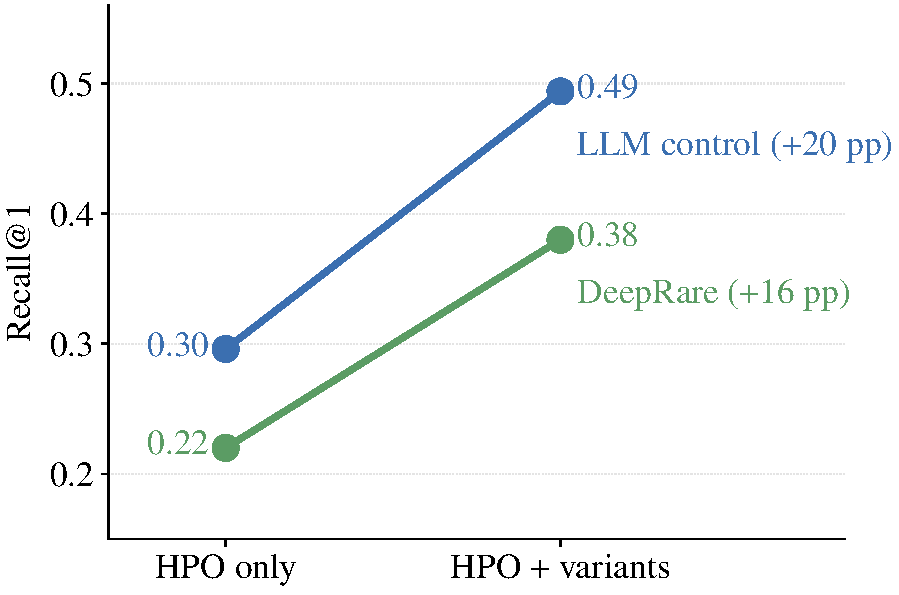
\includegraphics[width=0.86\linewidth]{Figure_supplementary/figH2_genotype.pdf}
\caption{H2 genotype channel. R@1 when the same cases are scored on phenotype
terms alone versus phenotype terms plus a structured variant block, for the
single-LLM control and for DeepRare; both gain about 16--20 points.}
\label{fig:h2genotype}
\end{figure}

\begin{figure}[h]
\centering
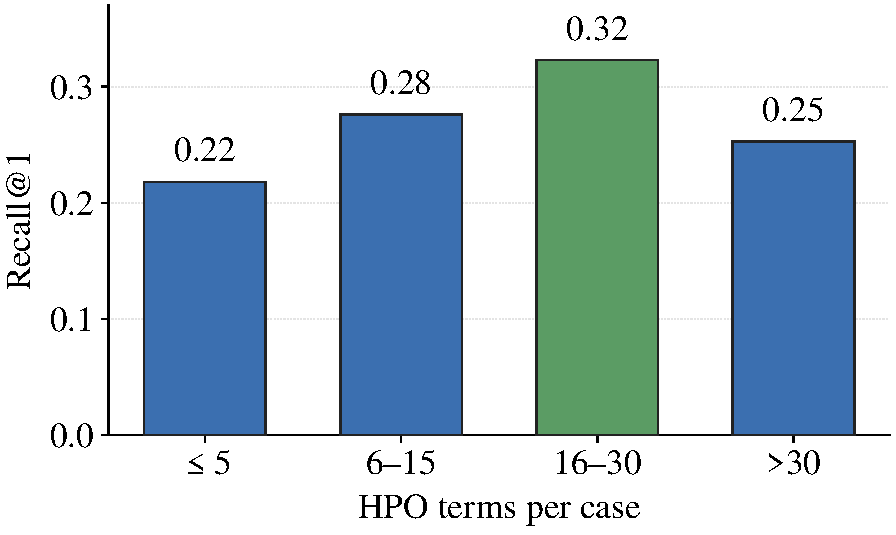
\includegraphics[width=0.86\linewidth]{Figure_supplementary/figM4_hpo_density.pdf}
\caption{H8 phenotype density. Pooled R@1 by the number of HPO terms per case;
the 16--30 band (highlighted) is the peak, an inverted-U consistent with too few
terms under-specifying and too many diluting the query.}
\label{fig:m4density}
\end{figure}

\begin{figure}[h]
\centering
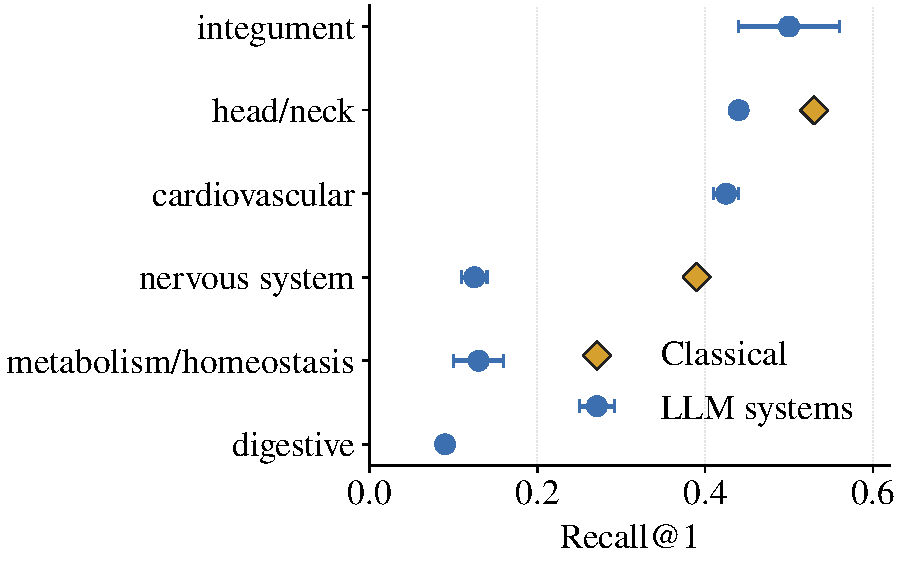
\includegraphics[width=0.86\linewidth]{Figure_supplementary/fig7_specialty_h7.pdf}
\caption{H7 specialty blind spots. R@1 by the case's modal HPO organ system.
Markers are the LLM systems (range shown as a whisker); diamonds mark the
classical baseline where it inverts the LLM ordering (nervous system, head/neck).}
\label{fig:h7specialty}
\end{figure}

% ======================================================================
\section{Cost Accounting}
\label{app:cost}

The evaluation comprises 97,985 predictions at a total API cost of \$297.89, or
\$0.0030 per prediction including offline runs. Per-prediction cost spans more
than an order of magnitude across backbones (Table~\ref{tab:cost},
Figure~\ref{fig:costbar}): GPT-5 minimal is the most expensive without a
consistent accuracy advantage, while V4-Flash is more than an order of magnitude
cheaper. Offline/classical baselines incur no API cost.

\begin{table}[h]
\centering
\scriptsize
\setlength{\tabcolsep}{4pt}
\caption{Per-prediction cost by backbone, and the multiple relative to the
cheapest backbone (V4-Flash). Offline/classical baselines incur no API cost.}
\label{tab:cost}
\begin{tabular}{@{}lrr@{}}
\toprule
Backbone & \$/prediction & $\times$ V4-Flash \\
\midrule
DS V4-Flash & 0.00032 & 1.0 \\
DS V4-Pro (reasoning-off) & 0.00098 & 3.1 \\
Gemini 3 Flash & 0.00341 & 10.7 \\
GPT-5 minimal & 0.00825 & 25.8 \\
LIRICAL / VC-RDAgent & 0.00000 & --- \\
\bottomrule
\end{tabular}
\end{table}

\begin{figure}[h]
\centering
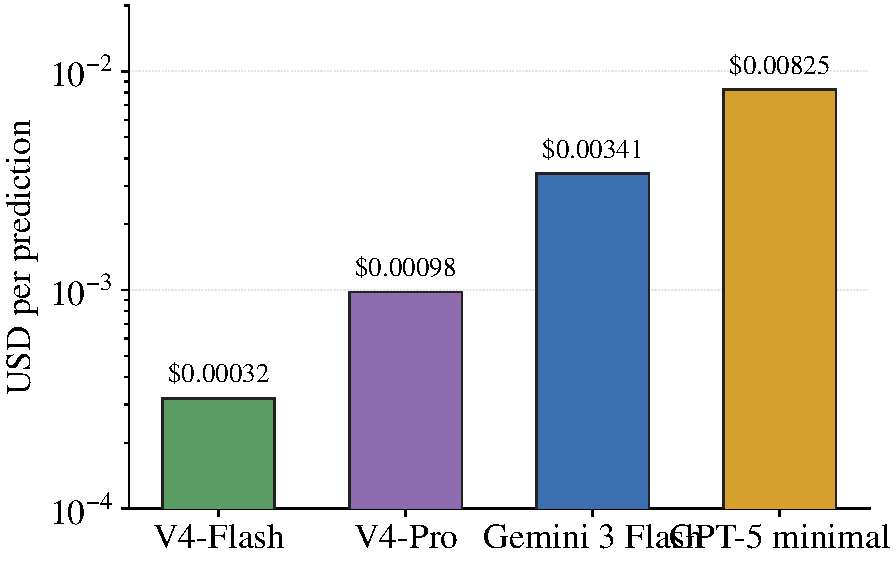
\includegraphics[width=\linewidth]{Figure_supplementary/fig_costbar.pdf}
\caption{Per-prediction API cost by backbone on a log scale. The cost ordering
does not induce a matching accuracy ordering (main paper, Figure~2b);
classical/offline baselines incur no API cost and are omitted from the log axis.}
\label{fig:costbar}
\end{figure}

% ======================================================================
\section{MIMIC-IV Note Probe}
\label{app:mimicnote}

The MIMIC-IV-Note probe uses the \emph{presentation} portion of a discharge
summary (chief complaint, history, exam, labs, imaging) as input, truncated
before any diagnosis-revealing section, with the gold disease name masked. This
avoids the answer-naming shortcut present when an ICD long-title is exposed. The
gold label remains code-derived (ICD$\rightarrow$Orphanet exact mapping), which we
flag as a code-supervision caveat; this probe is the MIMIC-IV-Note column of
Table~1 in the main paper.

\paragraph{Subset construction.}
The deterministic funnel is: 150,033 admissions with any ICD--ORPHA mapping
$\rightarrow$ 107,144 exact-mapped only (dropping 37,872 narrower-to-broader and
5,017 broader-to-narrower approximate maps) $\rightarrow$ 18,392 genuinely rare
gold $\rightarrow$ 2,325 where the rare disease is the admission's principal
diagnosis $\rightarrow$ 1,255 with a usable discharge summary (117 diseases,
sha256 \texttt{f5d9b437}\ldots) $\rightarrow$ 1,083 after dropping 172
prior-known mentions (112 diseases) $\rightarrow$ 855 in which the gold name
never appears verbatim (class A) $\rightarrow$ 687 after the strict Orphanet
synonym/abbreviation screen (105 diseases) $\rightarrow$ 416 restricted to
diseases carrying Orphanet disease-level HPO annotation (68 diseases, sha256
\texttt{67d156aa}\ldots), the frozen scored set. Prior-known detection uses a
$\pm45$-character window around each \texttt{[MASKED\_DIAGNOSIS]} token for
history cues (``history of'', ``hx'', ``known'', ``s/p'', ``diagnosed with'').
The synonym screen matters: 19.6\% of the nominally clean class-A notes still
contained a gold synonym or abbreviation that the crossmap-aware scorer credits
as a hit. Truncation alone left the gold name verbatim in only 2,776/78,166
(3.55\%) of notes, all subsequently masked; residual gold in
\texttt{model\_input} is 0 by programmatic assertion over the full set. The
funnel is itself a finding: only $\sim$1,255 admissions have ``a true rare
disease as the principal diagnosis with a usable note,'' quantifying the
validity limit of ICD-derived gold. A parallel capped line (${\leq}10$ cases per
disease, 359 cases / 105 diseases) is used where distribution balance matters
more than case count; 416 and 359 are both subsets of the 687 uncapped
strict-A set.

\paragraph{Contamination control (presentation vs.\ full note).}
Running an unscaffolded LLM on the same 416 cases twice---once on the full,
un-truncated, un-masked note and once on the masked presentation---isolates the
answer-naming shortcut. R@1 drops on all four backbones:
V4-Pro $0.500\!\rightarrow\!0.365$ ($-27\%$), V4-Flash
$0.553\!\rightarrow\!0.353$ ($-36\%$), GPT-5 $0.425\!\rightarrow\!0.363$
($-15\%$), Gemini $0.452\!\rightarrow\!0.373$ ($-18\%$); confidence intervals do
not overlap. Weaker models lose more, so the shortcut not only inflates absolute
scores but compresses and reorders the model ranking.

\paragraph{24-cell agent matrix.}
On the 416-case probe we ran six agent families across four backbones
(Table~\ref{tab:mimicmatrix}, mean micro-R@1 over backbones). The scaffolding
picture from the main HPO datasets replicates: the unscaffolded control ties the
best light-coordination scaffolds (MedAgents, MDAgents) within overlapping
intervals and far exceeds the heavier-orchestration systems, which collapse.
This is the second dataset behind the main-paper scaffolding figure. Every one of
the 24 cells is complete at 416/416; with the denominator fixed at 416, all
failures, timeouts, parser errors and empty-but-successful responses count as
misses (1,118 of 9,984 predictions, 11.2\%). Per-backbone cells are in Table~1 of
the main paper.

\begin{table}[h]
\centering
\scriptsize
\setlength{\tabcolsep}{5pt}
\caption{MIMIC-IV note probe: mean micro-R@1 over four backbones
(denominator 416; all failures counted as misses). Scoring is unified across
all cells.}
\label{tab:mimicmatrix}
\begin{tabular}{@{}lr@{}}
\toprule
Agent & Mean R@1 \\
\midrule
LLM control (no scaffold) & 0.364 \\
MDAgents & 0.367 \\
MedAgents & 0.350 \\
AgentClinic & 0.140 \\
DeepRare & 0.011 \\
MAI-DxO & 0.003 \\
\bottomrule
\end{tabular}
\end{table}

\paragraph{Honest boundaries.}
Gold is code-derived, not independent clinical adjudication; note coverage is
partial, so a selection bias between admissions with and without a discharge
summary cannot be excluded; and an organ-system stratification here is
disease-level (from the gold disease's Orphanet phenotype list), not
case-level, so it aligns structurally but not identically with the other
datasets; the 271 cases / 37 diseases dropped at the HPO step are an
annotation-coverage artifact of Orphanet \texttt{en\_product4} rather than a
quality filter, but they do narrow disease diversity. Finally, the screen is
name-based and case-level: a disease may remain inferable from a characteristic
treatment or laboratory pattern. These caveats bound what the MIMIC-IV-Note column
supports.

% ======================================================================
\section{Bootstrap and Reproducibility Notes}
\label{app:repro-notes}

All reported point estimates ship with bootstrap 95\% confidence intervals
(case-level bootstrap; percentile method). Several small per-agent and
per-backbone gaps fall within overlapping intervals and are not treated as
definitive rankings. Every confirmatory cell ships a reproducibility receipt
containing the run identifier, request identifiers when available, configuration
hash, denominator, failure breakdown, and cost. For LLM-judge evaluation of
free-text traces, we replay identical frozen traces across judges from different
model families, report judge-conditioned results rather than merged scores, and
chunk traces longer than 5,000 characters into overlapping 3,000-character
windows with 500-character overlap to prevent silent truncation. Deterministic
scoring is primary wherever a verifiable target exists; subjective trace scores
are reported as exploratory and, for consequential claims, audited against a
human-rated subset.

\end{document}
